
%% bare_jrnl.tex
%% V1.4b
%% 2015/08/26
%% by Michael Shell
%% see http://www.michaelshell.org/
%% for current contact information.
%%
%% This is a skeleton file demonstrating the use of IEEEtran.cls
%% (requires IEEEtran.cls version 1.8b or later) with an IEEE
%% journal paper.
%%
%% Support sites:
%% http://www.michaelshell.org/tex/ieeetran/
%% http://www.ctan.org/pkg/ieeetran
%% and
%% http://www.ieee.org/

%%*************************************************************************
%% Legal Notice:
%% This code is offered as-is without any warranty either expressed or
%% implied; without even the implied warranty of MERCHANTABILITY or
%% FITNESS FOR A PARTICULAR PURPOSE! 
%% User assumes all risk.
%% In no event shall the IEEE or any contributor to this code be liable for
%% any damages or losses, including, but not limited to, incidental,
%% consequential, or any other damages, resulting from the use or misuse
%% of any information contained here.
%%
%% All comments are the opinions of their respective authors and are not
%% necessarily endorsed by the IEEE.
%%
%% This work is distributed under the LaTeX Project Public License (LPPL)
%% ( http://www.latex-project.org/ ) version 1.3, and may be freely used,
%% distributed and modified. A copy of the LPPL, version 1.3, is included
%% in the base LaTeX documentation of all distributions of LaTeX released
%% 2003/12/01 or later.
%% Retain all contribution notices and credits.
%% ** Modified files should be clearly indicated as such, including  **
%% ** renaming them and changing author support contact information. **
%%*************************************************************************


% *** Authors should verify (and, if needed, correct) their LaTeX system  ***
% *** with the testflow diagnostic prior to trusting their LaTeX platform ***
% *** with production work. The IEEE's font choices and paper sizes can   ***
% *** trigger bugs that do not appear when using other class files.       ***                          ***
% The testflow support page is at:
% http://www.michaelshell.org/tex/testflow/



\documentclass[journal]{IEEEtran}
%
% If IEEEtran.cls has not been installed into the LaTeX system files,
% manually specify the path to it like:
% \documentclass[journal]{../sty/IEEEtran}





% Some very useful LaTeX packages include:
% (uncomment the ones you want to load)


% *** MISC UTILITY PACKAGES ***
%
%\usepackage{ifpdf}
% Heiko Oberdiek's ifpdf.sty is very useful if you need conditional
% compilation based on whether the output is pdf or dvi.
% usage:
% \ifpdf
%   % pdf code
% \else
%   % dvi code
% \fi
% The latest version of ifpdf.sty can be obtained from:
% http://www.ctan.org/pkg/ifpdf
% Also, note that IEEEtran.cls V1.7 and later provides a builtin
% \ifCLASSINFOpdf conditional that works the same way.
% When switching from latex to pdflatex and vice-versa, the compiler may
% have to be run twice to clear warning/error messages.




%\usepackage{color}

% *** CITATION PACKAGES ***
%
\usepackage{cite}
% cite.sty was written by Donald Arseneau
% V1.6 and later of IEEEtran pre-defines the format of the cite.sty package
% \cite{} output to follow that of the IEEE. Loading the cite package will
% result in citation numbers being automatically sorted and properly
% "compressed/ranged". e.g., [1], [9], [2], [7], [5], [6] without using
% cite.sty will become [1], [2], [5]--[7], [9] using cite.sty. cite.sty's
% \cite will automatically add leading space, if needed. Use cite.sty's
% noadjust option (cite.sty V3.8 and later) if you want to turn this off
% such as if a citation ever needs to be enclosed in parenthesis.
% cite.sty is already installed on most LaTeX systems. Be sure and use
% version 5.0 (2009-03-20) and later if using hyperref.sty.
% The latest version can be obtained at:
% http://www.ctan.org/pkg/cite
% The documentation is contained in the cite.sty file itself.



%\usepackage[section]{placeins}


% *** GRAPHICS RELATED PACKAGES ***
%
\ifCLASSINFOpdf
   \usepackage[pdftex]{graphicx}
  % declare the path(s) where your graphic files are
  % \graphicspath{{../pdf/}{../jpeg/}}
  % and their extensions so you won't have to specify these with
  % every instance of \includegraphics
  % \DeclareGraphicsExtensions{.pdf,.jpeg,.png}
\else
  % or other class option (dvipsone, dvipdf, if not using dvips). graphicx
  % will default to the driver specified in the system graphics.cfg if no
  % driver is specified.
  % \usepackage[dvips]{graphicx}
  % declare the path(s) where your graphic files are
  % \graphicspath{{../eps/}}
  % and their extensions so you won't have to specify these with
  % every instance of \includegraphics
  % \DeclareGraphicsExtensions{.eps}
\fi
% graphicx was written by David Carlisle and Sebastian Rahtz. It is
% required if you want graphics, photos, etc. graphicx.sty is already
% installed on most LaTeX systems. The latest version and documentation
% can be obtained at: 
% http://www.ctan.org/pkg/graphicx
% Another good source of documentation is "Using Imported Graphics in
% LaTeX2e" by Keith Reckdahl which can be found at:
% http://www.ctan.org/pkg/epslatex
%
% latex, and pdflatex in dvi mode, support graphics in encapsulated
% postscript (.eps) format. pdflatex in pdf mode supports graphics
% in .pdf, .jpeg, .png and .mps (metapost) formats. Users should ensure
% that all non-photo figures use a vector format (.eps, .pdf, .mps) and
% not a bitmapped formats (.jpeg, .png). The IEEE frowns on bitmapped formats
% which can result in "jaggedy"/blurry rendering of lines and letters as
% well as large increases in file sizes.
%
% You can find documentation about the pdfTeX application at:
% http://www.tug.org/applications/pdftex





% *** MATH PACKAGES ***
%
\usepackage{amsmath}
% A popular package from the American Mathematical Society that provides
% many useful and powerful commands for dealing with mathematics.
%
% Note that the amsmath package sets \interdisplaylinepenalty to 10000
% thus preventing page breaks from occurring within multiline equations. Use:
%\interdisplaylinepenalty=2500
% after loading amsmath to restore such page breaks as IEEEtran.cls normally
% does. amsmath.sty is already installed on most LaTeX systems. The latest
% version and documentation can be obtained at:
% http://www.ctan.org/pkg/amsmath


\usepackage{epsfig}


% *** SPECIALIZED LIST PACKAGES ***
%
%\usepackage{algorithmic}
% algorithmic.sty was written by Peter Williams and Rogerio Brito.
% This package provides an algorithmic environment fo describing algorithms.
% You can use the algorithmic environment in-text or within a figure
% environment to provide for a floating algorithm. Do NOT use the algorithm
% floating environment provided by algorithm.sty (by the same authors) or
% algorithm2e.sty (by Christophe Fiorio) as the IEEE does not use dedicated
% algorithm float types and packages that provide these will not provide
% correct IEEE style captions. The latest version and documentation of
% algorithmic.sty can be obtained at:
% http://www.ctan.org/pkg/algorithms
% Also of interest may be the (relatively newer and more customizable)
% algorithmicx.sty package by Szasz Janos:
% http://www.ctan.org/pkg/algorithmicx




% *** ALIGNMENT PACKAGES ***
%
%\usepackage{array}
% Frank Mittelbach's and David Carlisle's array.sty patches and improves
% the standard LaTeX2e array and tabular environments to provide better
% appearance and additional user controls. As the default LaTeX2e table
% generation code is lacking to the point of almost being broken with
% respect to the quality of the end results, all users are strongly
% advised to use an enhanced (at the very least that provided by array.sty)
% set of table tools. array.sty is already installed on most systems. The
% latest version and documentation can be obtained at:
% http://www.ctan.org/pkg/array


% IEEEtran contains the IEEEeqnarray family of commands that can be used to
% generate multiline equations as well as matrices, tables, etc., of high
% quality.

%
%\usepackage{array}

% *** SUBFIGURE PACKAGES ***
\ifCLASSOPTIONcompsoc
  \usepackage[caption=false,font=normalsize,labelfont=sf,textfont=sf]{subfig}
\else
  \usepackage[caption=false,font=footnotesize]{subfig}
\fi
% subfig.sty, written by Steven Douglas Cochran, is the modern replacement
% for subfigure.sty, the latter of which is no longer maintained and is
% incompatible with some LaTeX packages including fixltx2e. However,
% subfig.sty requires and automatically loads Axel Sommerfeldt's caption.sty
% which will override IEEEtran.cls' handling of captions and this will result
% in non-IEEE style figure/table captions. To prevent this problem, be sure
% and invoke subfig.sty's "caption=false" package option (available since
% subfig.sty version 1.3, 2005/06/28) as this is will preserve IEEEtran.cls
% handling of captions.
% Note that the Computer Society format requires a larger sans serif font
% than the serif footnote size font used in traditional IEEE formatting
% and thus the need to invoke different subfig.sty package options depending
% on whether compsoc mode has been enabled.
%
% The latest version and documentation of subfig.sty can be obtained at:
% http://www.ctan.org/pkg/subfig




% *** FLOAT PACKAGES ***
%
%\usepackage{fixltx2e}
% fixltx2e, the successor to the earlier fix2col.sty, was written by
% Frank Mittelbach and David Carlisle. This package corrects a few problems
% in the LaTeX2e kernel, the most notable of which is that in current
% LaTeX2e releases, the ordering of single and double column floats is not
% guaranteed to be preserved. Thus, an unpatched LaTeX2e can allow a
% single column figure to be placed prior to an earlier double column
% figure.
% Be aware that LaTeX2e kernels dated 2015 and later have fixltx2e.sty's
% corrections already built into the system in which case a warning will
% be issued if an attempt is made to load fixltx2e.sty as it is no longer
% needed.
% The latest version and documentation can be found at:
% http://www.ctan.org/pkg/fixltx2e


%\usepackage{stfloats}
% stfloats.sty was written by Sigitas Tolusis. This package gives LaTeX2e
% the ability to do double column floats at the bottom of the page as well
% as the top. (e.g., "\begin{figure*}[!b]" is not normally possible in
% LaTeX2e). It also provides a command:
%\fnbelowfloat
% to enable the placement of footnotes below bottom floats (the standard
% LaTeX2e kernel puts them above bottom floats). This is an invasive package
% which rewrites many portions of the LaTeX2e float routines. It may not work
% with other packages that modify the LaTeX2e float routines. The latest
% version and documentation can be obtained at:
% http://www.ctan.org/pkg/stfloats
% Do not use the stfloats baselinefloat ability as the IEEE does not allow
% \baselineskip to stretch. Authors submitting work to the IEEE should note
% that the IEEE rarely uses double column equations and that authors should try
% to avoid such use. Do not be tempted to use the cuted.sty or midfloat.sty
% packages (also by Sigitas Tolusis) as the IEEE does not format its papers in
% such ways.
% Do not attempt to use stfloats with fixltx2e as they are incompatible.
% Instead, use Morten Hogholm'a dblfloatfix which combines the features
% of both fixltx2e and stfloats:
%
% \usepackage{dblfloatfix}
% The latest version can be found at:
% http://www.ctan.org/pkg/dblfloatfix




%\ifCLASSOPTIONcaptionsoff
%  \usepackage[nomarkers]{endfloat}
% \let\MYoriglatexcaption\caption
% \renewcommand{\caption}[2][\relax]{\MYoriglatexcaption[#2]{#2}}
%\fi
% endfloat.sty was written by James Darrell McCauley, Jeff Goldberg and 
% Axel Sommerfeldt. This package may be useful when used in conjunction with 
% IEEEtran.cls'  captionsoff option. Some IEEE journals/societies require that
% submissions have lists of figures/tables at the end of the paper and that
% figures/tables without any captions are placed on a page by themselves at
% the end of the document. If needed, the draftcls IEEEtran class option or
% \CLASSINPUTbaselinestretch interface can be used to increase the line
% spacing as well. Be sure and use the nomarkers option of endfloat to
% prevent endfloat from "marking" where the figures would have been placed
% in the text. The two hack lines of code above are a slight modification of
% that suggested by in the endfloat docs (section 8.4.1) to ensure that
% the full captions always appear in the list of figures/tables - even if
% the user used the short optional argument of \caption[]{}.
% IEEE papers do not typically make use of \caption[]'s optional argument,
% so this should not be an issue. A similar trick can be used to disable
% captions of packages such as subfig.sty that lack options to turn off
% the subcaptions:
% For subfig.sty:
% \let\MYorigsubfloat\subfloat
% \renewcommand{\subfloat}[2][\relax]{\MYorigsubfloat[]{#2}}
% However, the above trick will not work if both optional arguments of
% the \subfloat command are used. Furthermore, there needs to be a
% description of each subfigure *somewhere* and endfloat does not add
% subfigure captions to its list of figures. Thus, the best approach is to
% avoid the use of subfigure captions (many IEEE journals avoid them anyway)
% and instead reference/explain all the subfigures within the main caption.
% The latest version of endfloat.sty and its documentation can obtained at:
% http://www.ctan.org/pkg/endfloat
%
% The IEEEtran \ifCLASSOPTIONcaptionsoff conditional can also be used
% later in the document, say, to conditionally put the References on a 
% page by themselves.




% *** PDF, URL AND HYPERLINK PACKAGES ***
%
%\usepackage{url}
% url.sty was written by Donald Arseneau. It provides better support for
% handling and breaking URLs. url.sty is already installed on most LaTeX
% systems. The latest version and documentation can be obtained at:
% http://www.ctan.org/pkg/url
% Basically, \url{my_url_here}.




% *** Do not adjust lengths that control margins, column widths, etc. ***
% *** Do not use packages that alter fonts (such as pslatex).         ***
% There should be no need to do such things with IEEEtran.cls V1.6 and later.
% (Unless specifically asked to do so by the journal or conference you plan
% to submit to, of course. )


% correct bad hyphenation here
\hyphenation{op-tical net-works semi-conduc-tor}


\begin{document}
%
% paper title
% Titles are generally capitalized except for words such as a, an, and, as,
% at, but, by, for, in, nor, of, on, or, the, to and up, which are usually
% not capitalized unless they are the first or last word of the title.
% Linebreaks \\ can be used within to get better formatting as desired.
% Do not put math or special symbols in the title.
\title{Tailored object detection methods for trail cameras}
%
%
% author names and IEEE memberships
% note positions of commas and nonbreaking spaces ( ~ ) LaTeX will not break
% a structure at a ~ so this keeps an author's name from being broken across
% two lines.
% use \thanks{} to gain access to the first footnote area
% a separate \thanks must be used for each paragraph as LaTeX2e's \thanks
% was not built to handle multiple paragraphs
%

\author{First author,
	second author,
	third author, 
	and Alastair~Frank,
	\thanks{R. S. C. Winter  is with the Electrical and Computer Engineering Department, University of Alberta, Edmonton, AB T6G 2V4, Canada (e-mail: rswinter@ualberta.ca).\newline
		Kevin Hawkshaw, Erik Hedlin and Alastair Frank are with the Department of Biological Sciences, University of Alberta, Edmonton, AB T6G 2V4, Canada (e-mail: hawkshaw@ualberta.ca,hedlin@ualberta.ca,kfranke@ualberta.ca). 
	}% <-this % stops a space
%\thanks{J. Doe and J. Doe are with Anonymous University.}% <-this % stops a space
\thanks{Manuscript received XXX, XXXX; revised XXX, XXXX.}}

% note the % following the last \IEEEmembership and also \thanks - 
% these prevent an unwanted space from occurring between the last author name
% and the end of the author line. i.e., if you had this:
% 
% \author{....lastname \thanks{...} \thanks{...} }
%                     ^------------^------------^ not want these spaces!
%
% a space would be appended to the last name and could cause every name on that
% line to be shifted left slightly. This is one of those "LaTeX things". For
% instance, "\textbf{A} \textbf{B}" will typeset as "A B" not "AB". To get
% "AB" then you have to do: "\textbf{A}\textbf{B}"
% \thanks is no different in this regard, so shield the last } of each \thanks
% that ends a line with a % and do not let a space in before the next \thanks.
% Spaces after \IEEEmembership other than the last one are OK (and needed) as
% you are supposed to have spaces between the names. For what it is worth,
% this is a minor point as most people would not even notice if the said evil
% space somehow managed to creep in.



% The paper headers
\markboth{Submitted to}%
{Shell \MakeLowercase{\textit{et al.}}: Bare Demo of IEEEtran.cls for IEEE Journals}
% The only time the second header will appear is for the odd numbered pages
% after the title page when using the twoside option.
% 
% *** Note that you probably will NOT want to include the author's ***
% *** name in the headers of peer review papers.                   ***
% You can use \ifCLASSOPTIONpeerreview for conditional compilation here if
% you desire.




% If you want to put a publisher's ID mark on the page you can do it like
% this:
%\IEEEpubid{0000--0000/00\$00.00~\copyright~2015 IEEE}
% Remember, if you use this you must call \IEEEpubidadjcol in the second
% column for its text to clear the IEEEpubid mark.



% use for special paper notices
%\IEEEspecialpapernotice{(Invited Paper)}




% make the title area
\maketitle

% As a general rule, do not put math, special symbols or citations
% in the abstract or keywords.
\begin{abstract}
Motion sensor camera traps are used extensively in the fields of zoology and ecology. 	Camera traps have been around for decades and have revolutionized wildlife research and conservation due to their ability to capture information with little expense, and minimal disturbance to the wildlife. Recently, the ability of computers to recognize certain aspects of images has led to the use of these techniques to save human time in examining the camera trap images. In this work object detection methods are applied to peregrine nest cameras. Our application of these techniques is able to achieve XX\% accuracy. Additionally due to the nature of the sequence of images taken, any mistakes made can be rectified by using a time-sequence of the data. 
	
	
%This paper investigates the near field characteristics of radiators and the impact of the near field on synthetic aperture radar (SAR) imaging. The pulse properties are studied in the near field; including the velocities of the pulse peak, pulse envelope peak, and the centrovelocity. A method for the experimental characterization of transceivers is presented. The characteristics of the transceivers can then be taken into account during the image reconstruction leading to higher accuracy imaging in the near field. Near field imaging is then conducted in several different situations and the antenna characterization is then compared to conventional imaging without the use of the actual speeds of pulse propagation. 

%Several  The pulse reshaping in the near field is studied. The pulse velocities; pulse peak, pulse envelope peak, and centrovelocity are found for a specific transceiver arrangement. These velocity profiles are then used to improve image quality in (SAR) imaging and the reconstruction using the global back projection algorithm. 
\end{abstract}

% Note that keywords are not normally used for peerreview papers.
\begin{IEEEkeywords}
Deep learning, Animal identification, Camera-trap images, Constitutional Neural Networks
\end{IEEEkeywords}






\IEEEpeerreviewmaketitle



\section{Introduction}


\IEEEPARstart{S}{urprisingly} the concept of a camera trap has been around since the 1890s~\cite{harris2010automatic}. However camera traps would not find significant use for over a century later. Cameras traps have since been used increasingly by researchers to record and track different biological phenomena~\cite{o2010camera}. With the increase of the technolical ability of camera trap in the 1990s led to a flood of research. They have been used to study nest ecology~\cite{major1994inexpensive}, vertebrate activity~\cite{carthew1991monitoring}, rare species identification~\cite{surridge1999striped}, research of rare individuals~\cite{martyr1997important}, population estimation~\cite{o2006estimating}, and survivorship~\cite{karanth2006assessing} among many others. 

Camera traps have become more popular and have become a important piece of a lot of zoological research because it enables researchers to collect data inexpensively, in-obstructively, and with high frequency~\cite{o2010camera}. This has led to the rapid expansion of the use of camera traps in research. As more research makes use of camera traps, difficulties dealing with the analysis of the data has arisen. The authors of~\cite{harris2010automatic} identified four problems restricting the use of camera trap in research: (1) cataloging imagery is slow and usually lags behind acquisition, (2) user entry is tedious and can be error prone, (3) inconsistent filing complicated data analysis and sharing, and (4) the struggle to keep pace with analysis and data management restricts the deployment of additional cameras. In~\cite{harris2010automatic} the solution presented is a systematic procedure of analysis, making use of different computer programs to help in the organization of the data. 

However, systematic organization still requires the time of an expert to analyze the images. Not only does this tie up researchers from other tasks, but limits the number of cameras due to the shear number of images to be processed. With the advancement of computer vision techniques, several works have been done to make use of this to automatically identify images. Initially many techniques made use of hand-designed features to classify animals~\cite{swinnen2014novel}. Most recently, deep learning has emerged as the most powerful computer vision technique. It has shown ability to solve many computer image problems and is able to surpass human experts in many ways.  Deep learning has been used to distinguish birds from mammals~\cite{gomez2016animal} as well as in larger class problems such as~\cite{chen2014deep}. Some of the best results were obtained on the SS data-set. Authors in~\cite{villa2017towards} obtained a 57\% correct in species identification of a 26 class subset of the data. Authors in~\cite{norouzzadeh2018automatically} extended these results by obtaining 92\% accuracy despite taking into account the full 48 class problem. 

In comparison to this previous work, we apply DNN to relatively smaller problems, having at most three classes. The camera traps are nest-sites. Although less complicated than large class problems, we show higher quality in terms of class identification with significantly reduced training examples. Using the characteristics of the cameras which take three consecutive images during a motion event, allows the already high results to be supplemented and a large percent of the mistakes to be rectified creating a near expert level quality allowing completely automated image analysis and production of results. In addition, the nest cameras contain more movement and information than trail cameras, for example for the 28 cameras in 2015, the project captured over 2.1 million photos, making up 841 GB of information. Thus the different aspects of the situation requires a modified solution. 

Most biological research groups will not have significant computational resources available. This would be even more notable in the nest traps, due to the shear number of images produced. Thus computational aspects should be taken into account. YOLOv3~\cite{redmon2018yolov3} is a DNN which is designed to run fast than comparative techniques. This has a trade-off of quality and it has been shown to have slightly lower scores than other techniques such as XXX~\cite{redmon2018yolov3}. 

In Section~\ref{articraptorssection} the arctic raptors project is introduced. Section~\ref{section:procedure} outlines the steps taken in the training and implementation of the computer vision techniques. Section~\ref{section:timeanalysis} describes the use of the time series of data to correct possible errors in object detection. Finally the paper is concluded in Section~\ref{sectionconclusion}.  





\begin{figure}[!tb]
	\centering
	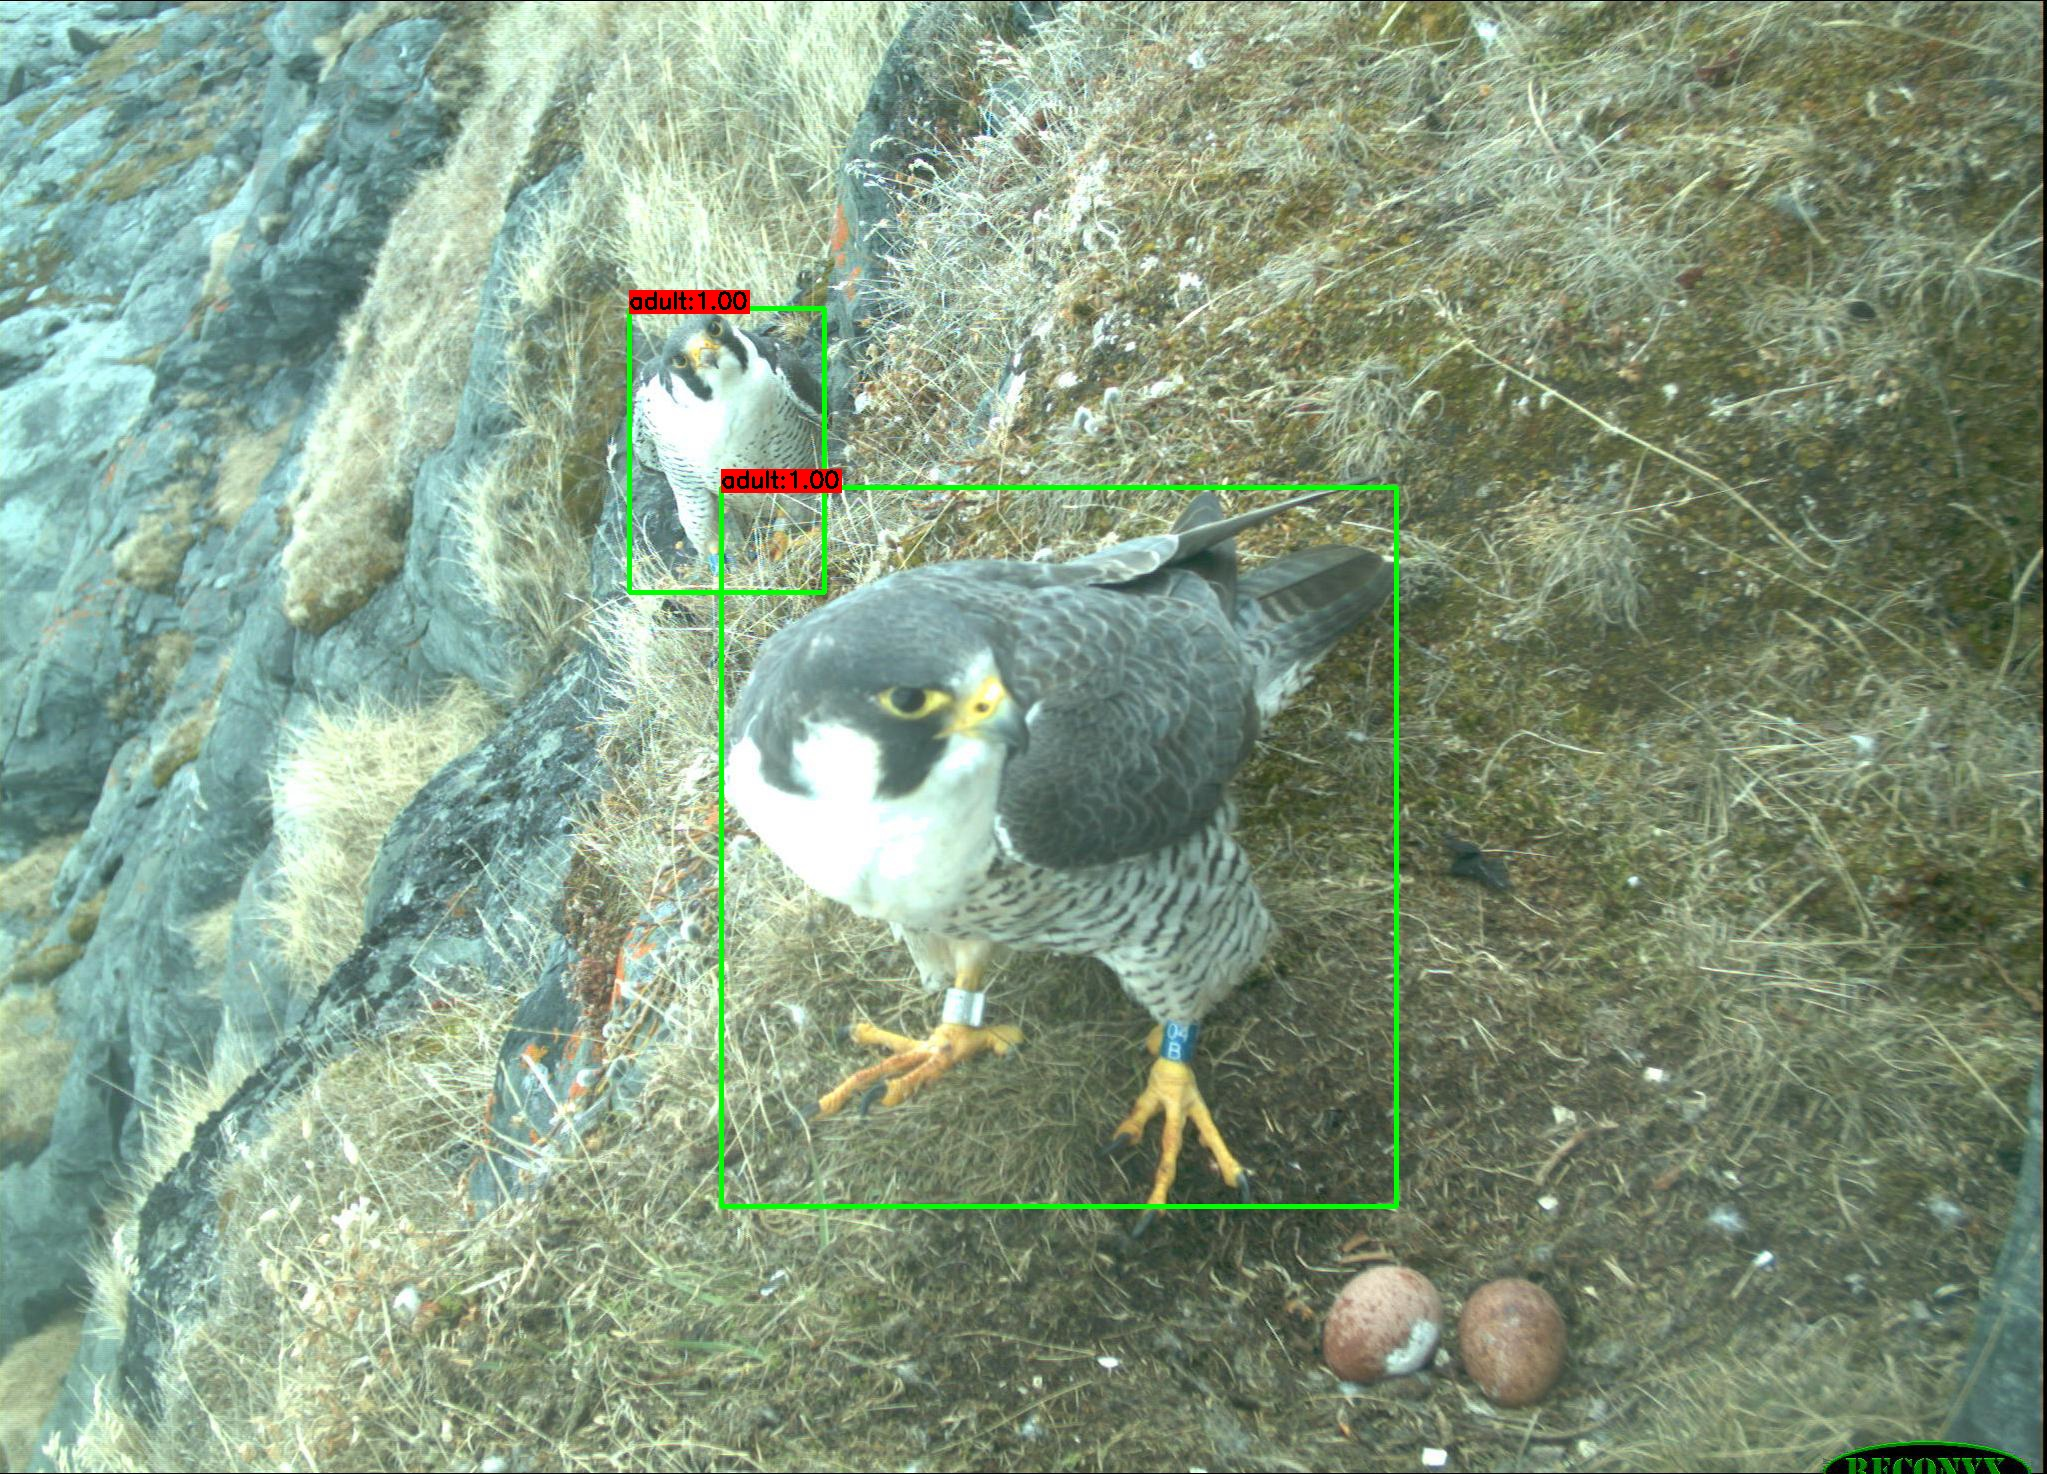
\includegraphics[width=3.5in]{adults.jpg}
	\caption{Adults detection.}
	\label{adults}
\end{figure}

\begin{figure}[!tb]
	\centering
	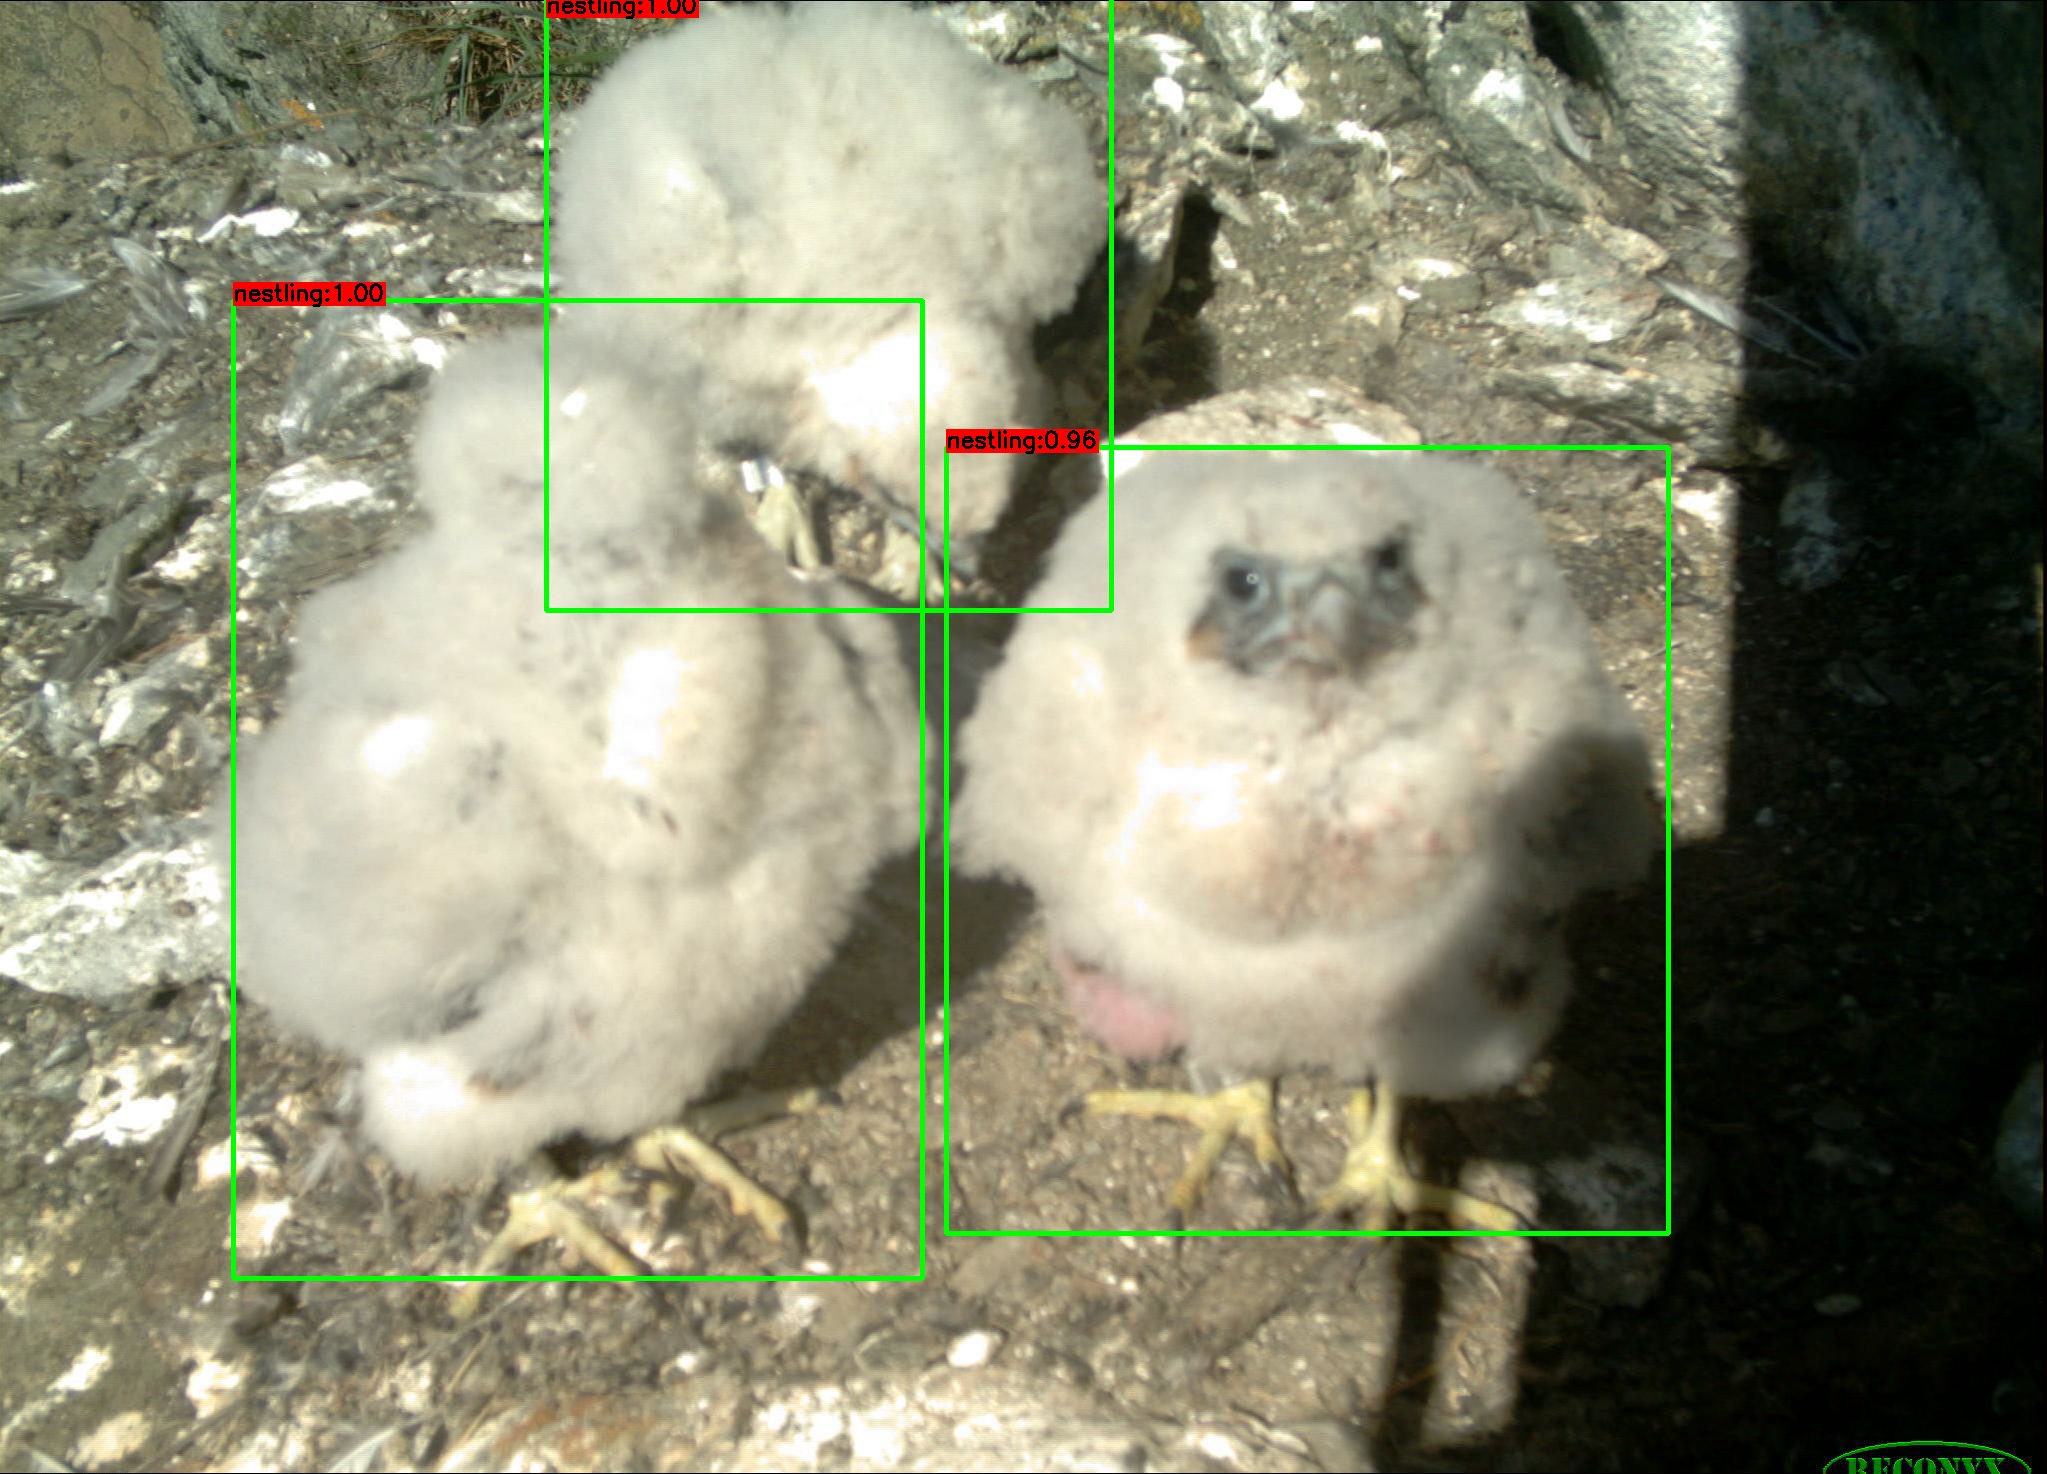
\includegraphics[width=3.5in]{nestlings.jpg}
	\caption{Detection of nestlings}
	\label{nestlings}
\end{figure}


\begin{figure}[!tb]
	\centering
	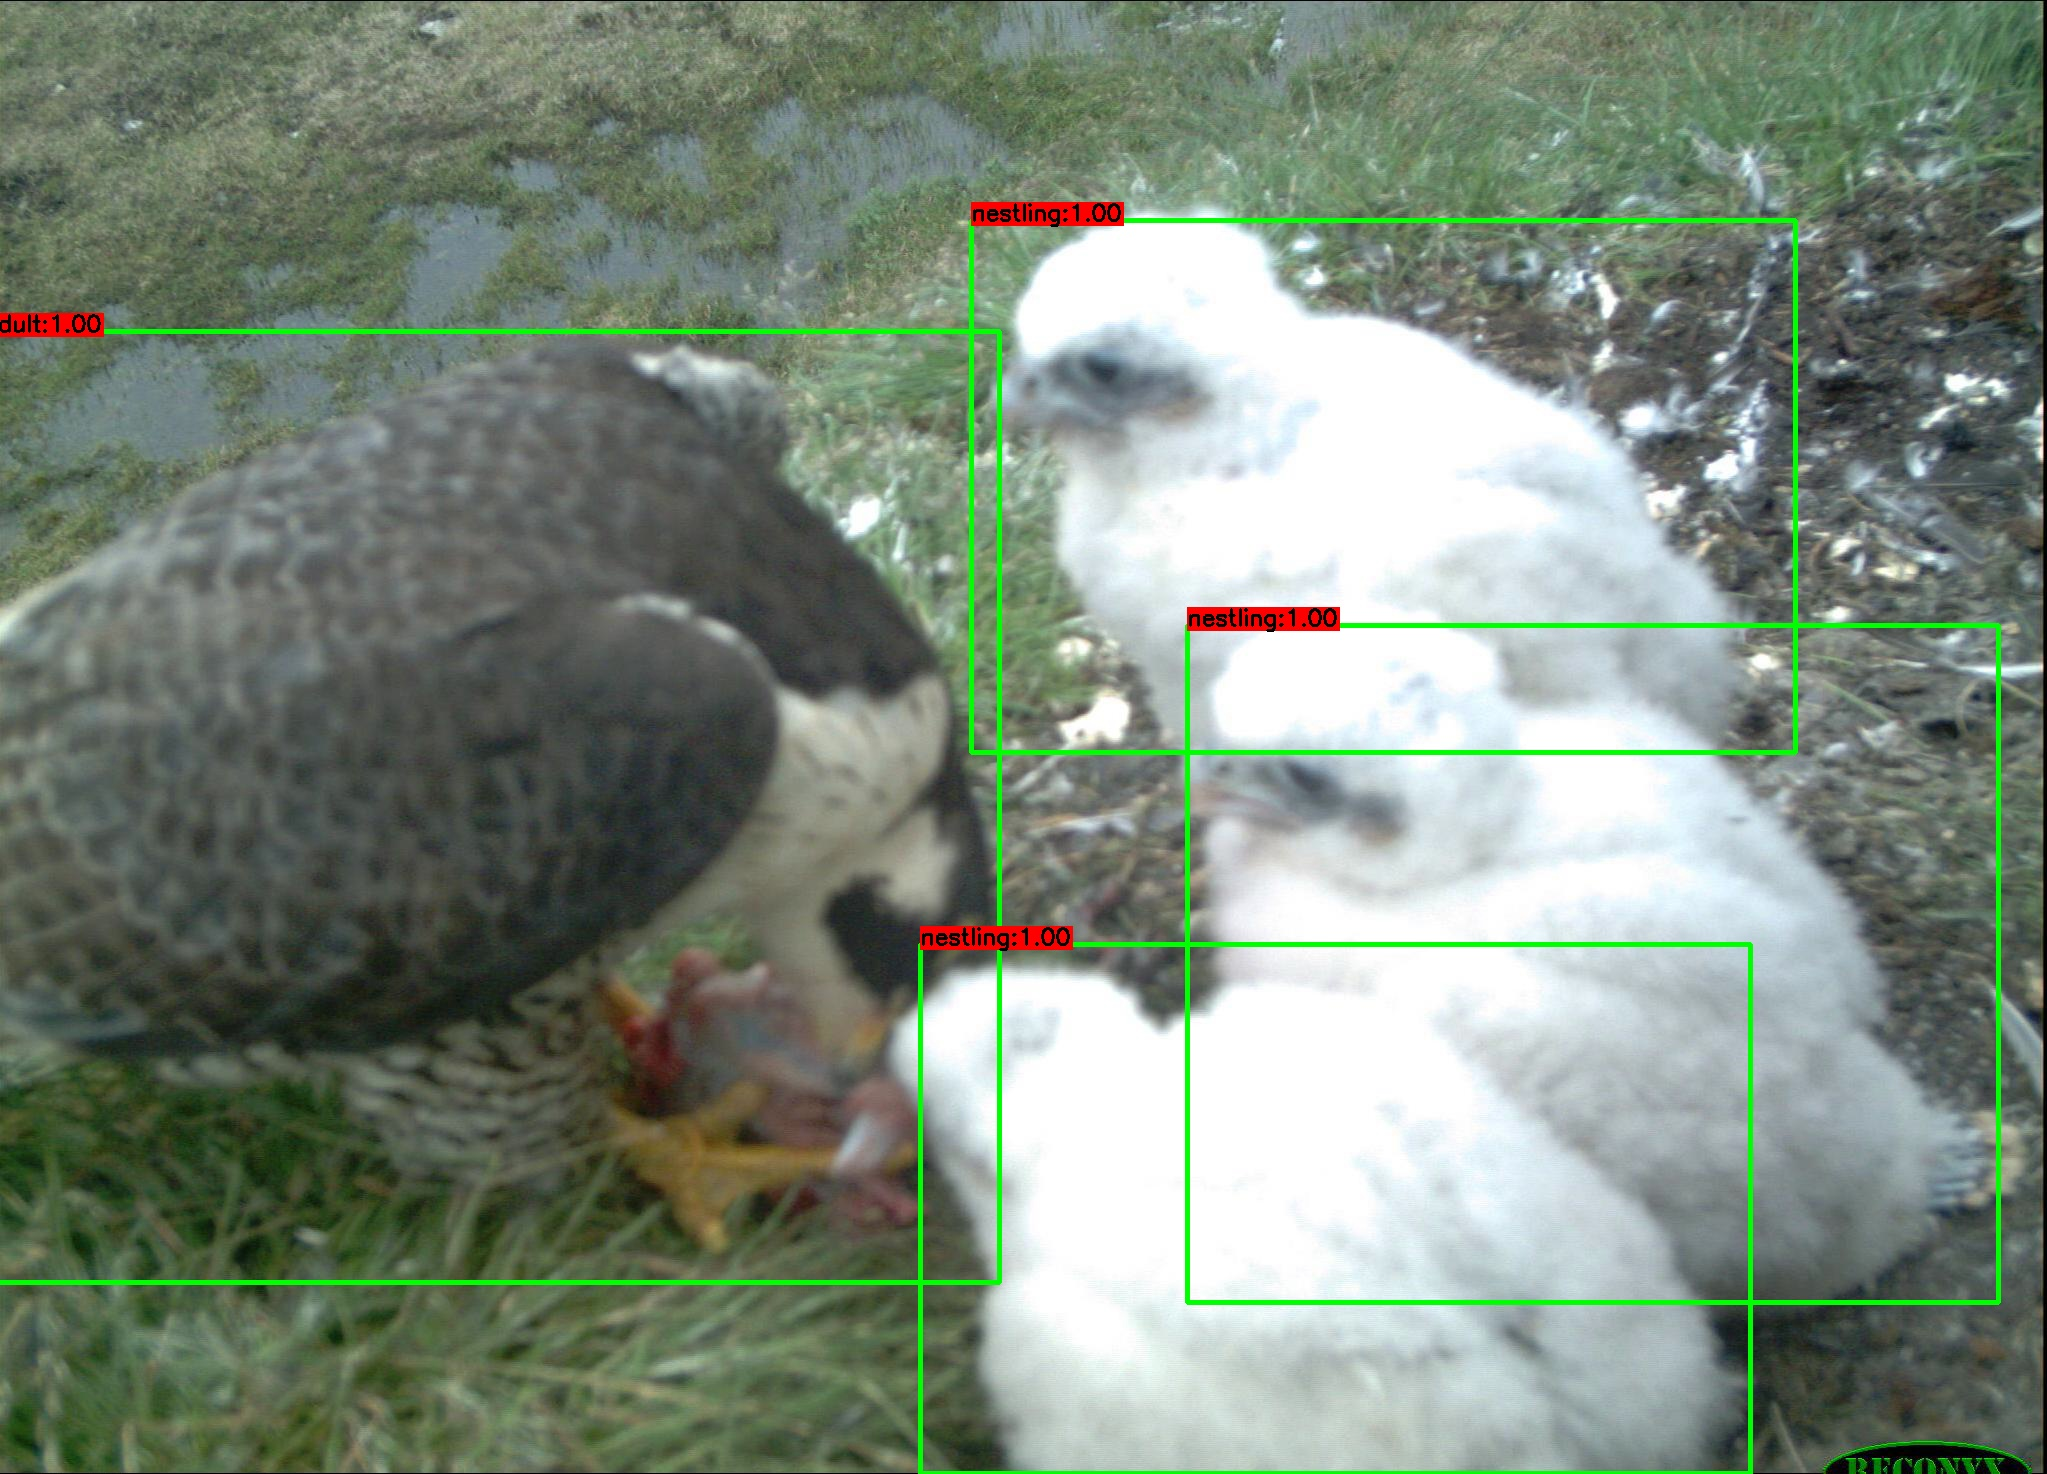
\includegraphics[width=3.5in]{bothnestlingadults.jpg}
	\caption{Detection showing nestlings and adults.}
	\label{bothnestlingsadults}
\end{figure}


\begin{figure}[!tb]
	\centering
	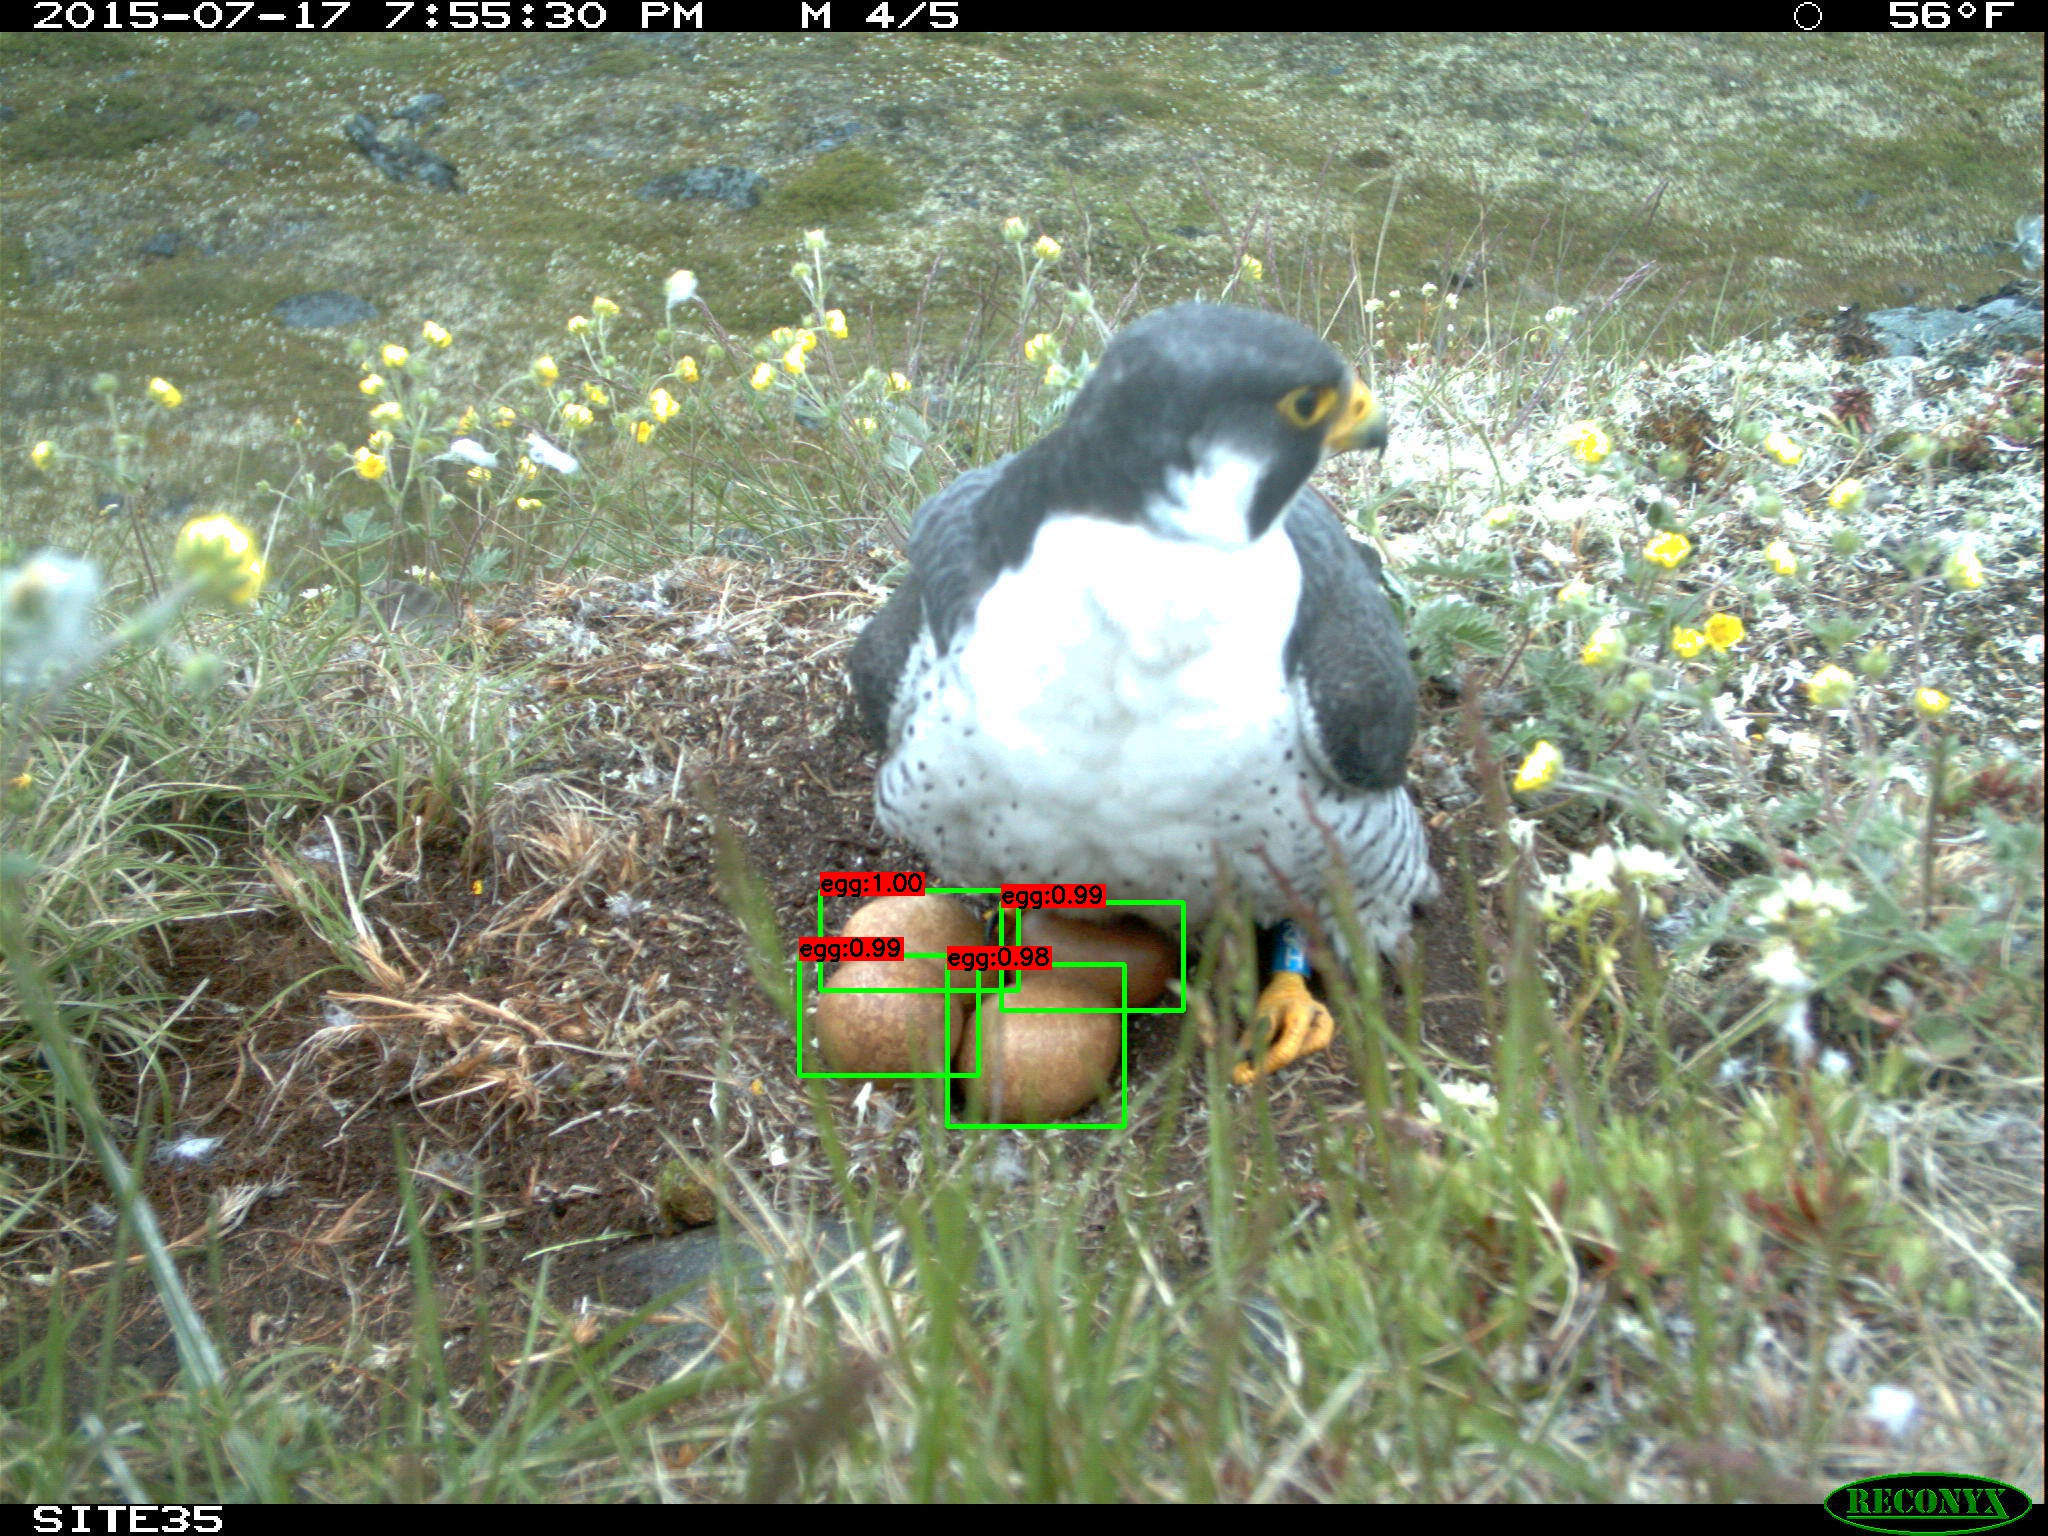
\includegraphics[width=3.5in]{eggs.jpg}
	\caption{Egg detection.}
	\label{eggs}
\end{figure}

\begin{figure}[!tb]
	\centering
	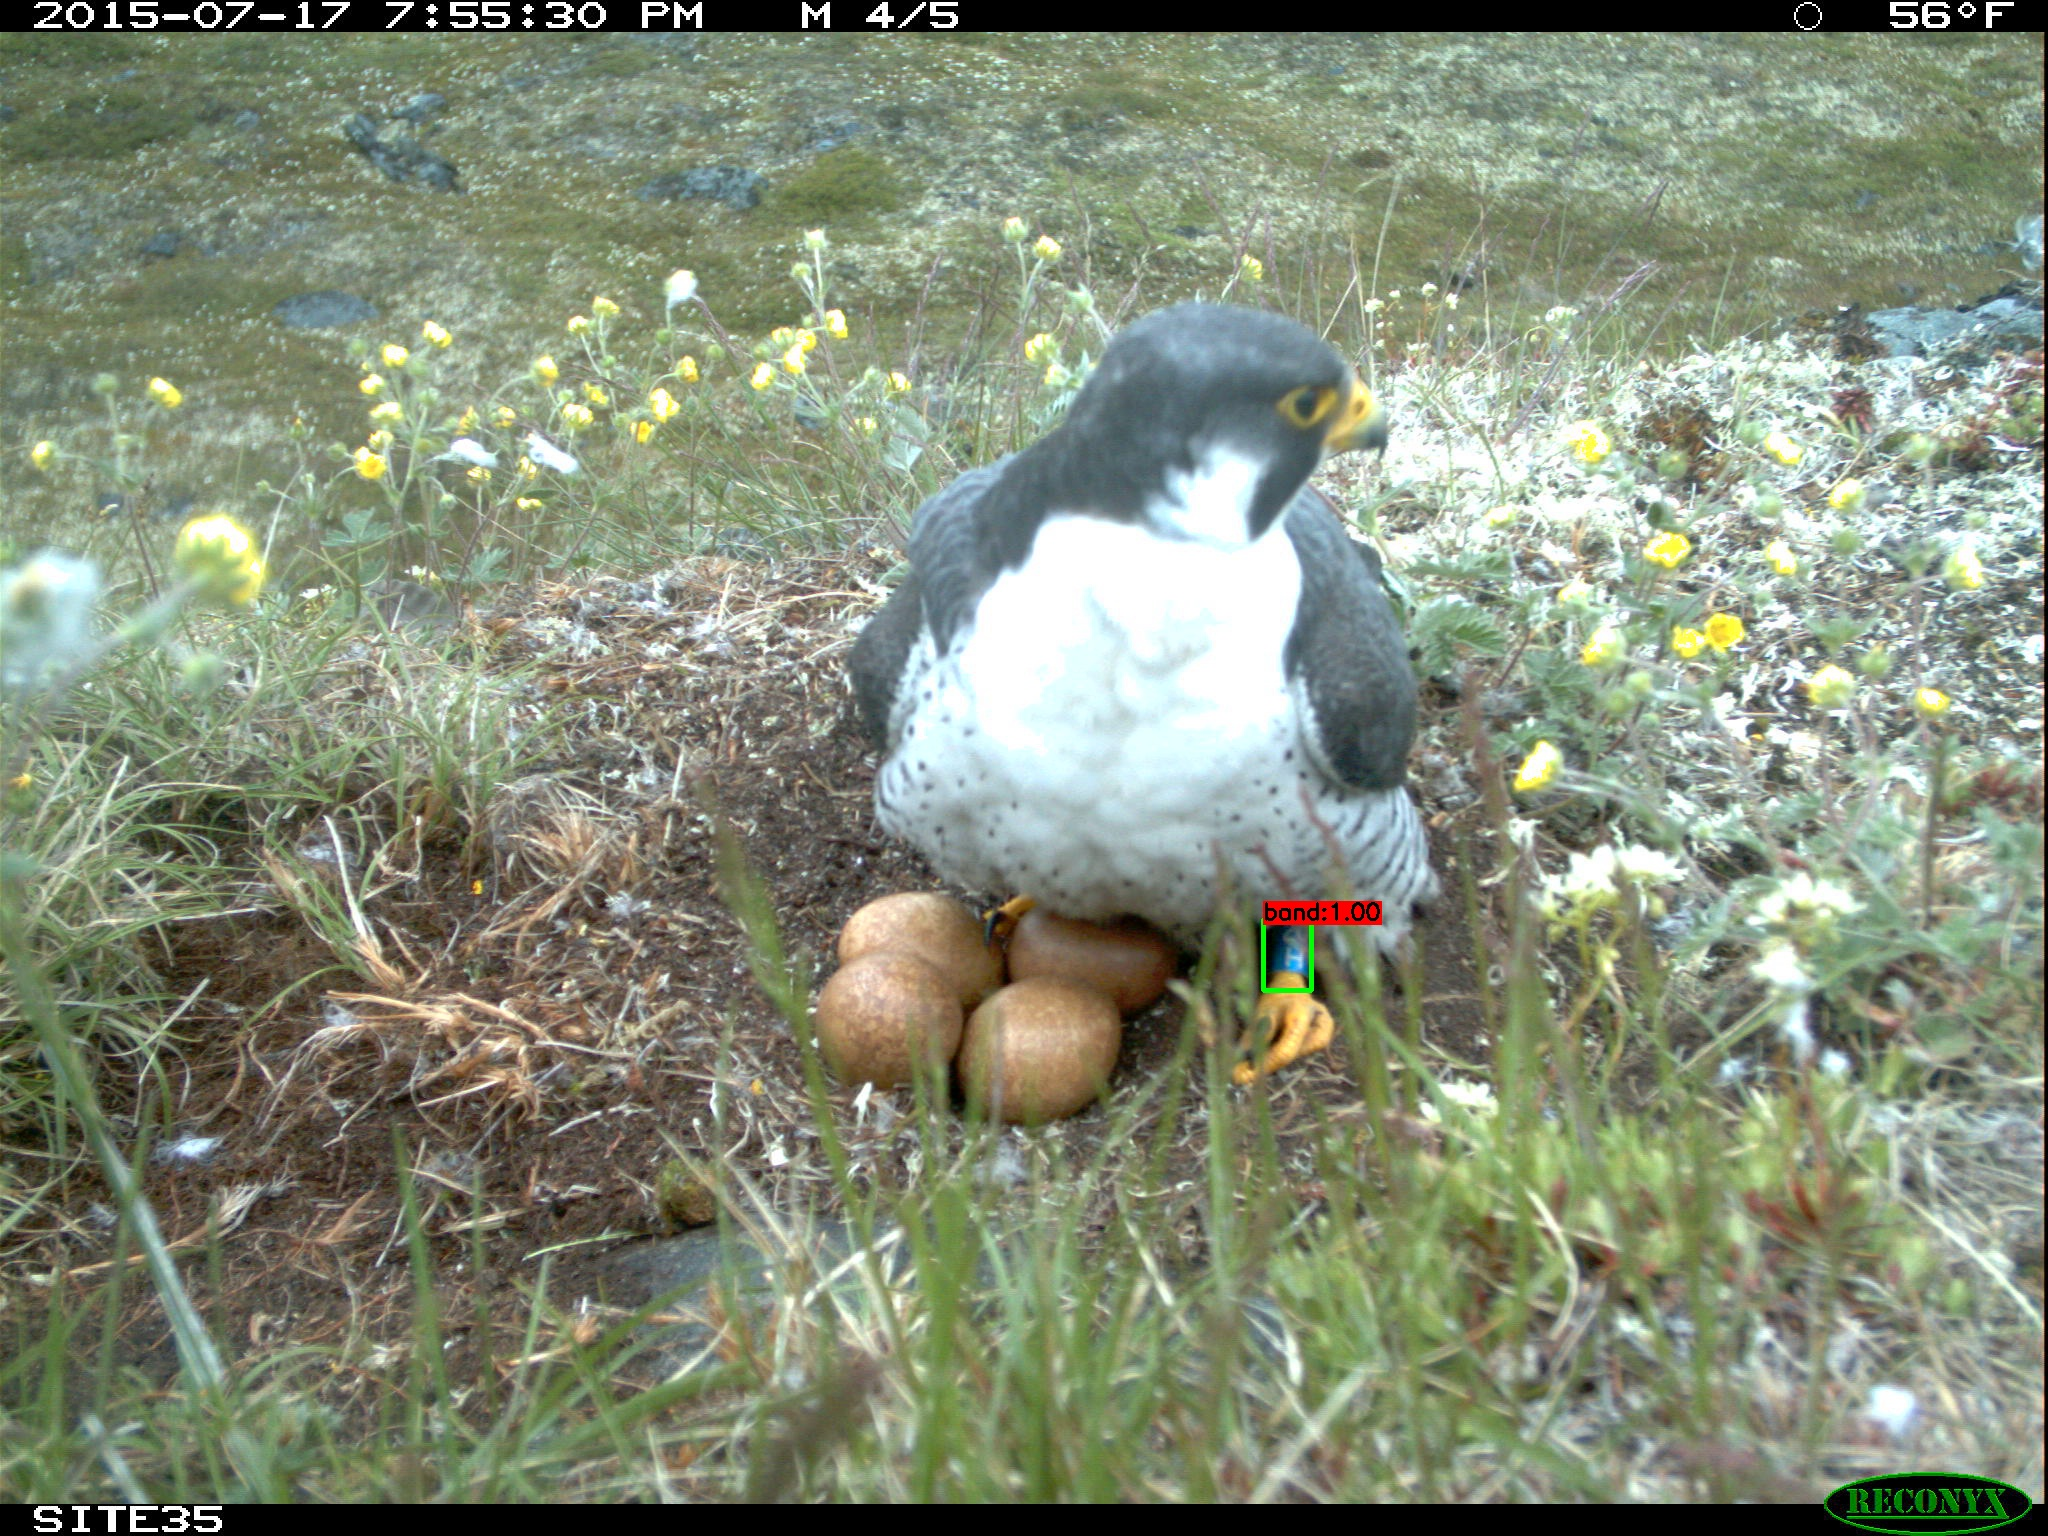
\includegraphics[width=3.5in]{band.jpg}
	\caption{Band detection.}
	\label{band}
\end{figure}

\begin{figure}[!tb]
	\centering
	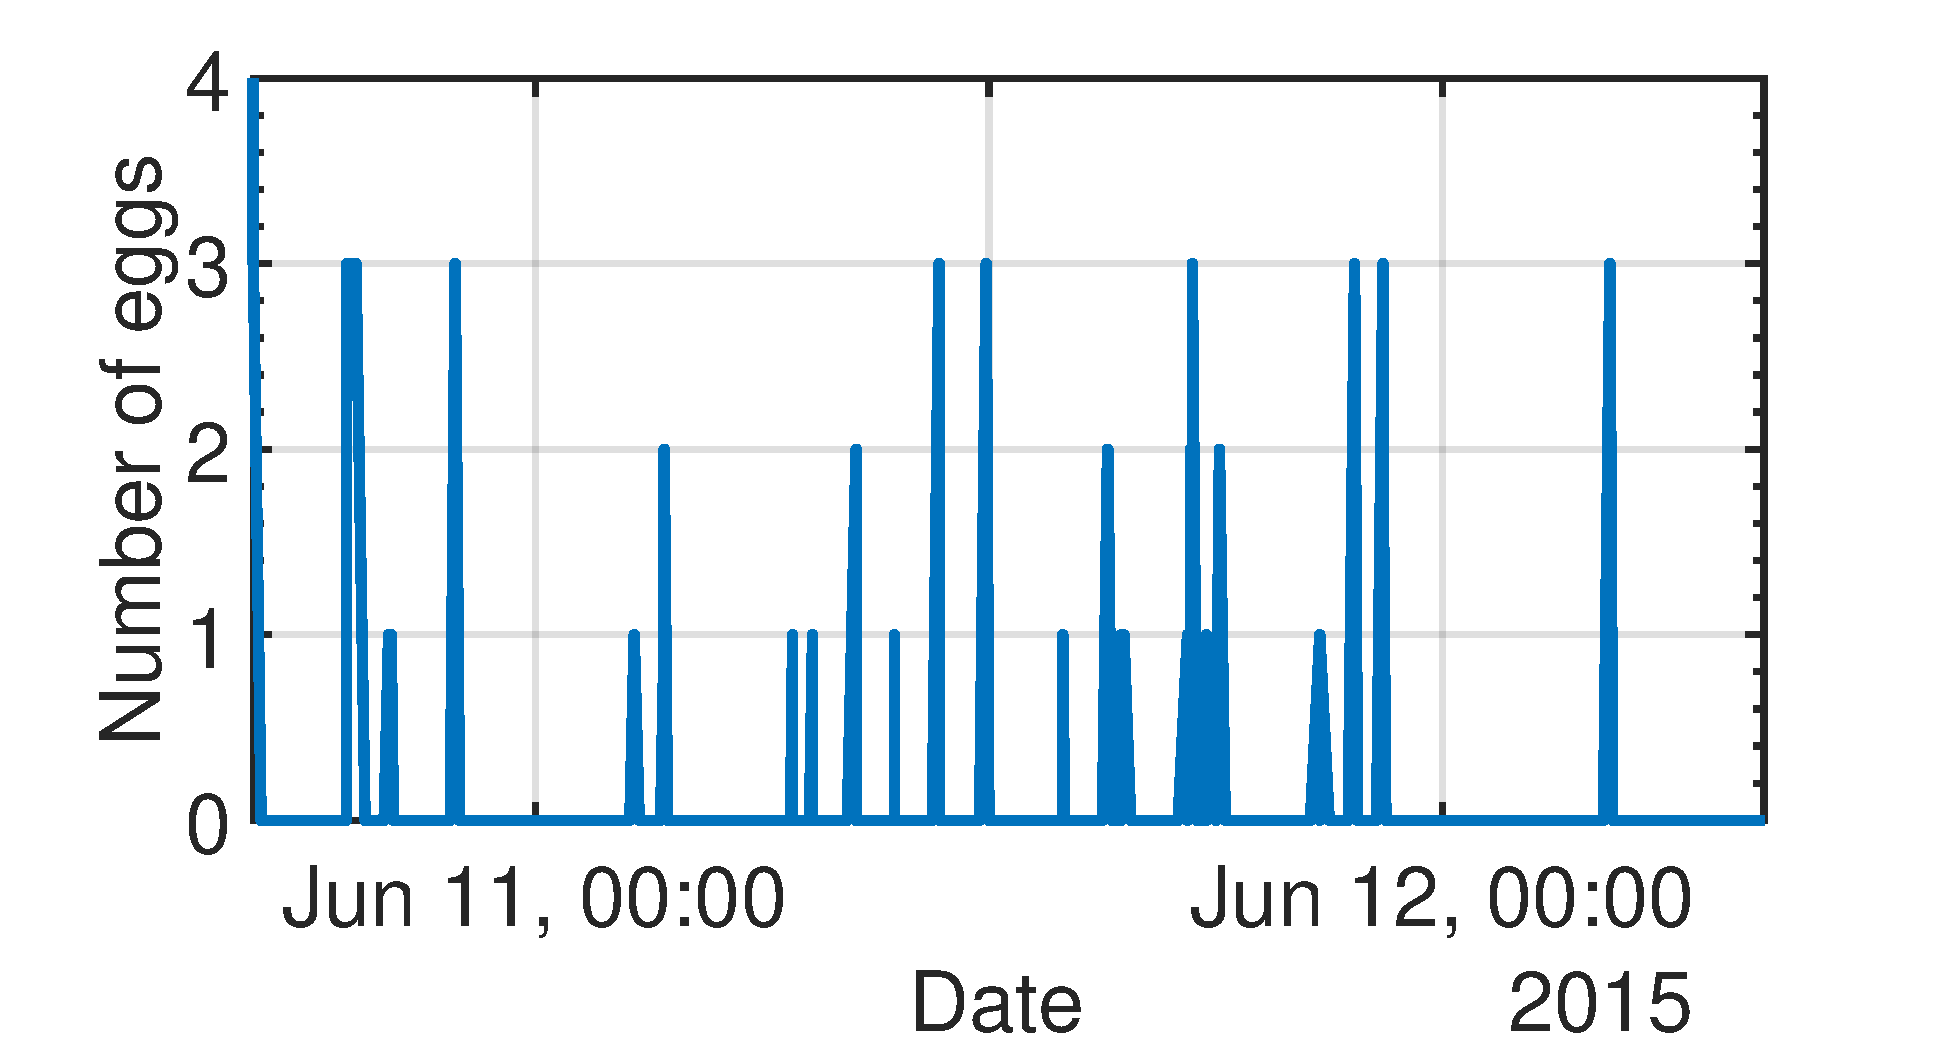
\includegraphics[width=3.5in]{eggsovertime.pdf}
	\caption{Number of eggs detected over time. This value can be used to determine the incubating behavior.}
	\label{eggsovertime}
\end{figure}

\section{Arctic Raptors}\label{articraptorssection}
The arctic raptors research group is a longterm research project studying peregrine falcons in Arctic Canada. The primary study area consists of the region of Rankin Inlet, Nunavut. Positioned on the west coast of Hudsons Bay, and is home to the densest known population of Peregrine falcons in the arctic. The project is headed by the University of Alberta and the University of Quebec at Rimouski, and is a project member of ArcticNet network. One of the research areas is the nesting program. This involves the study of the survival rate and nesting behavior of the raptors. The study involves 36 camera traps, each consisting of a camera aimed at a potential or suspected nesting site. The cameras consist of Reconyx HP2X cameras. The cameras are set to acquire one photo every 15 minutes and three photos one second apart in the case the camera is triggered by motion. 

At the beginning of the arctic raptors project, researchers in the field would visit the nests on a daily basis and track the nestling survivability and behavior~\cite{}. When camera traps were applied they allowed a much better understanding of the mortality, if a nest was taken by a fox sometime between researchers visit, it could now be known. 

Some problems of interest that could be automated could be the amount of time parents spend on the nest, the hatching dates, the nestling mortality. 

%Arctic Raptors is a research group headed by Dr. Alastair Franke (University of Alberta) dedicated to the study of Peregrine Falcons and other raptors in arctic Canada. Our primary study area surrounds the community of Rankin Inlet, Nunavut on the west coast of Hudson Bay, which is home to the densest known population of Peregrine Falcons in the arctic. The research group is made up of students from from both the University of Alberta and the University of Quebec at Rimouski, and is a project member of ArcticNet network of scientists and managers from around Canada.

\section{Methods}\label{section:procedure}
For the problems of interest which where outlined in Section~\ref{articraptorssection} can be solved using object detection of a three class problem. Where eggs, adult birds, and nestlings, bands are the four classes. Different numbers of images for the different classes were obtained from the dataset for training purposes. This set consisted of 91 images with bands, 106 images with eggs, and 450 images containing either adults and nestlings. These images were augmented with bounding boxes of the objects of interest and then the training for the darknet training was undertaken. Thanks to the relative size of the class number, the training converged rapidly towards a high quality result. 

\section{Results}\label{section:results}

\subsection{Time analysis}\label{section:timeanalysis}
The cameras used in this study take three pictures when detecting motion as well as a image every 15 minutes if no motion is detected. This time series data can be used to increase the correct decisions made when examining a single image. Firstly, the adult birds are larger and move through more of the frame at any point. Therefore, depending on the nestlings age, a motion event can be more likely attributed to the presence of an adult. Additionally, in a motion event three images can be used to see if an adult is present. The motion event usually takes the form of an adult coming to the nest, a feeding event, or an adult leaving the nest. Thus if the three images contain an adult in the first two images and no detection in the third image, that might indicate that the adult has left the nest site. If the next image taken 15 minutes later, also contains a low probability of an adult, together these results can be added together to make a conclusion on what event took place.  






\section{Conclusion}\label{sectionconclusion}

This paper demonstrates the high accuracy of quality of results from trail cameras used in conjunction with convolution deep learning methods. Due to limited class size and high correlated training sets, the results demonstrate a XX\% overall accuracy rate. Due to the nature of the cameras, which take three photos in rapid succession during a motion trigger event, the time series data can be used to increase the quality of the results further, to XX\%. For many research groups who have more homogeneous environments and a limited number of classes these techniques could be easily modified for their use. Although training of a DNN generally requires significant computational resources, making use of YOLOv3 minimizes the computational burden during image analysis, making this a possibility for a larger number of biological based research groups. 



%
\bibliography{mybib}
\bibliographystyle{ieeetr}
%


\end{document}


